% ============================================================
% Paper 2: Context-Aware Adaptive Perception for Mixed Traffic
% Author : Trọng Nghĩa
% Target : ICRA 2027 (primary) / IEEE IV 2027 (backup)
%          CONFERENCE format — 6–8 pages incl. references.
% NOTE   : Using IEEEtran [conference]. The official ICRA kit ships
%          ieeeconf.cls — swap the documentclass line when the ICRA 2027
%          author kit is released; the body is compatible with both.
% ============================================================
\documentclass[conference]{IEEEtran}
\IEEEoverridecommandlockouts

% ── Packages ────────────────────────────────────────────────
\usepackage[T1]{fontenc}
\usepackage[utf8]{inputenc}
\usepackage{amsmath, amssymb}
\usepackage{graphicx}
\usepackage{tikz}
\usetikzlibrary{arrows.meta,positioning,calc}
\usepackage{booktabs}           % professional tables (\toprule etc.)
\usepackage{multirow}
\usepackage{algorithm}
\usepackage{algpseudocode}
\usepackage{cite}               % IEEE-style [1]–[3] compression
\usepackage{xcolor}
\usepackage{subcaption}
\usepackage[hidelinks]{hyperref}

% Draft-only TODO marker — remove before submission.
\newcommand{\todo}[1]{\textcolor{red}{[TODO: #1]}}

% ── Metadata ────────────────────────────────────────────────
\title{\LARGE \bf Context-Aware Adaptive Perception for Motorcycle-Dominant
       Mixed Traffic: Dual-Task Detection and Tracking}

% Names in ASCII to stay within T1 fontenc; add full Vietnamese
% diacritics later via the vntex/T5 route if desired.
% Student emails share the st.ueh.edu.vn domain → grouped {a, b}@domain
% (standard IEEE idiom); mentor's email on its own line.
\author{%
\IEEEauthorblockN{Le~Trong~Nghia, Vo~Xuan~Lanh, and Nguyen~Thien~Bao}
\IEEEauthorblockA{University of Economics Ho Chi Minh City (UEH),
                  Ho Chi Minh City, Vietnam\\
\texttt{\{nghiale.31241024698,~lanhvo.31241025950\}@st.ueh.edu.vn},
\texttt{baont@ueh.edu.vn}}
}

% ── Document ────────────────────────────────────────────────
\begin{document}

\maketitle
\thispagestyle{empty}
\pagestyle{empty}

%% ── Abstract ──────────────────────────────────────────────
\begin{abstract}
  % ── Abstract ─────────────────────────────────────────────────────────
% Target: 150–200 words. [R] numbers filled after real-footage ablation.
% ─────────────────────────────────────────────────────────────────────
Perception pipelines for urban traffic surveillance typically rely on
fixed detection thresholds and a single linear motion model, and both
assumptions break down in motorcycle-dominant mixed traffic: dense
weaving maneuvers fragment tracks, and static thresholds produce
persistent false-positive accident alerts.
%
We propose a context-aware adaptive perception pipeline with three
components: (C1)~a lightweight context estimator that reads traffic
density, time of day, image brightness, and recent false-positive rate,
and adjusts detector confidence, tracker buffer length, and motion-model
selection online with hysteresis-stabilized switching; (C2)~a
class-conditioned motion model that tracks motorcycles with a constant
turn-rate and velocity (CTRV) extended Kalman filter while other vehicle
classes retain the standard linear filter; and (C3)~a dual-task track
reliability score that serves high-precision accident alerting and
high-recall multi-agent signal-control observations from a single
pipeline via two task-specific thresholds.
%
On hand-annotated ground truth from a self-collected Vietnamese urban
dataset, C2 improves motorcycle identity preservation over a
YOLO11+ByteTrack baseline for $0.85$\,ms of additional per-frame tracker
latency, and improves both detection precision and recall simultaneously
--- something no per-frame confidence threshold can do.
We quantify the sensitivity of the identity gain to residual annotation
error rather than reporting a single figure.
We further show that C2's components are not separable: uncertainty-gated
re-association \emph{alone} degrades identity, and only becomes effective
once confidence-scaled measurement noise makes the filter's uncertainty
estimate trustworthy.
We report negatively on the remaining components --- context adaptation
does not improve on a calibrated fixed threshold in the single traffic
regime our annotated segment covers, and the reliability score is too
weakly discriminative (AUC $0.609$) to filter usefully once C2 has
removed most spurious tracks --- and identify what each would require to
be validated.

\end{abstract}

%% ── Sections ──────────────────────────────────────────────
% ── Section I: Introduction ──────────────────────────────────────────
% Conference budget: ~0.75 page.
% NOTE (citation audit, kept from earlier pass): WHO 2023 supports
% "motorcycles dominant + majority of deaths in Viet Nam", NOT a precise
% "94% modal share" figure. Add a VN-specific source if a percentage is
% needed (see references.bib open items).
% ─────────────────────────────────────────────────────────────────────

\section{Introduction}
\label{sec:intro}

Vietnam has one of the highest road-traffic fatality burdens in
Southeast Asia; motorcycles are the dominant vehicle type and are
involved in the majority of road-traffic
deaths~\cite{WHO2023_roadsafety}.
Automated surveillance systems that detect accidents in real time and
supply high-quality observations to adaptive signal control are
therefore of practical urgency.
Modern perception pipelines combine a single-stage detector (e.g.,
YOLO11~\cite{Khanam2024_yolo11}) with a multi-object tracker (e.g.,
ByteTrack~\cite{Zhang2022_bytetrack}), yet two systematic failures
emerge when they operate in motorcycle-dominant mixed traffic.

First, \emph{track fragmentation}: during dense weaving maneuvers,
motorcycles occlude each other at irregular angles, and the linear
Kalman filter used by mainstream trackers coasts along a straight line
through the occlusion while the hidden motorcycle keeps turning --- the
track is lost or re-identified with a new identity, degrading the
observations consumed by downstream multi-agent controllers.
Second, \emph{false-positive accident alerts}: with a fixed confidence
threshold, sudden braking, sharp lane changes, and cluster occlusions
are misclassified as accidents, flooding operators with spurious
alerts.
Both failures share one root cause: thresholds and motion models are
\emph{static}, unable to adapt to rush-hour density, nighttime
low-contrast lighting, or the class-specific dynamics of two-wheeled
vehicles.

Prior systems do not bridge this gap.
Commercial platforms such as Hikvision AID~\cite{Hikvision_AID} target
highway, car-only scenarios.
Academic trackers such as StrongSORT~\cite{Du2023_strongsort} and
recent occlusion-aware designs~\cite{Hashempoor2025_fasttracker} retain
a single linear motion model for all classes.
Context-aware detection work adapts to weather or
illumination~\cite{Liu2022_iayolo} but considers neither
class-conditioned motion dynamics nor the requirements of multiple
downstream tasks.

We address these limitations with a \emph{context-aware adaptive
perception} pipeline for motorcycle-dominant mixed traffic.
A lightweight context estimator continuously reads four signals ---
vehicle density, time of day, image brightness, and recent
false-positive rate --- and adjusts detection confidence and tracking
hyperparameters online.
A class-conditioned motion model tracks motorcycles with a constant
turn-rate and velocity (CTRV) extended Kalman filter, explicitly
capturing weaving dynamics, while cars, buses, and trucks retain the
standard linear filter.
A dual-task reliability score then lets one pipeline serve both
high-precision accident alerting and high-recall signal-control
observations without task-specific retuning.

\noindent\textbf{Contributions.}
\begin{itemize}
  \item \textbf{C1 --- Context estimator and adaptive parameter
        controller:} four traffic-context signals drive the detector
        confidence threshold, tracker buffer length, and motion-model
        selection per frame, with EMA smoothing and hysteresis to
        prevent parameter oscillation (Sec.~\ref{subsec:c1}).
  \item \textbf{C2 --- Class-conditioned CTRV motion model:} a
        motorcycle-specific extended Kalman filter with state
        $[x, y, v, \theta, \omega]^\top$ integrated into ByteTrack,
        reducing fragmentation during high-curvature maneuvers
        (Sec.~\ref{subsec:c2}).
  \item \textbf{C3 --- Dual-task track reliability score:} a
        lightweight combination of track age, detection consistency,
        motion smoothness, and class stability, split by two
        task-specific thresholds for accident-alert precision and
        multi-agent observation recall (Sec.~\ref{subsec:c3}).
\end{itemize}

We evaluate on a self-collected Vietnamese urban dataset with an
ablation over all three components, plus controlled synthetic studies
isolating the motion model
(Secs.~\ref{sec:experiments}--\ref{sec:results}).

% ── Section II: Related Work ─────────────────────────────────────────
% Conference budget: ~0.75 page. Three threads + positioning paragraph.
% TODO before submission: add 1–2 recent (2024–2026) accident-detection
% and adaptive-perception citations per thread; see references.bib.
% ─────────────────────────────────────────────────────────────────────

\section{Related Work}
\label{sec:related}

\subsection{Accident Detection in Traffic Surveillance}
\label{subsec:rw_accident}

Vision-based accident detection is commonly formulated as clip- or
frame-level classification over surveillance footage.
The CADP dataset~\cite{Shah2018_cadp} established CCTV-based accident
analysis; D2-City~\cite{Che2019_d2city} provides large-scale dashcam
footage of diverse (including Chinese urban) traffic.
Deployed commercial systems such as Hikvision AID~\cite{Hikvision_AID}
detect incidents on highways with car-centric assumptions.
Across this line of work, classifiers run with fixed operating points
tuned offline on pre-segmented clips; none adapts its thresholds to the
traffic state it currently observes, which is precisely the regime in
which false alerts accumulate in dense mixed traffic.

\subsection{Multi-Object Tracking in Urban Scenes}
\label{subsec:rw_mot}

Tracking-by-detection dominates modern MOT.
SORT~\cite{Bewley2016_sort} paired a linear Kalman filter with
IoU-based Hungarian association; ByteTrack~\cite{Zhang2022_bytetrack}
improved recall by also associating low-score detections;
StrongSORT~\cite{Du2023_strongsort} strengthened appearance cues; and
recent occlusion-aware trackers exploit scene
structure~\cite{Hashempoor2025_fasttracker}.
Benchmarks such as MOT20~\cite{Dendorfer2020_mot20} focus on
pedestrians and cars, whose image-plane motion is well served by a
constant-velocity assumption.
All of these trackers apply one linear motion model to every object
class.
Nonlinear models with an explicit turn-rate state, notably CTRV,
were shown to outperform constant-velocity models for maneuvering
vehicles in the sensor-fusion literature~\cite{Schubert2008_ctrv}, yet
class-conditioned motion modeling --- and motorcycle weaving in
particular --- remains unaddressed in tracking-by-detection MOT.

\subsection{Context-Aware and Adaptive Perception}
\label{subsec:rw_adaptive}

Adaptive perception work mostly targets environmental domain shift:
Image-Adaptive YOLO~\cite{Liu2022_iayolo} learns image-enhancement
parameters for adverse weather, and related methods adjust
preprocessing or confidence calibration for night or rain.
These approaches adapt to \emph{appearance} conditions but leave the
tracker's hyperparameters and motion assumptions fixed, and they
optimize a single downstream objective.
Serving two tasks with conflicting operating points --- precision-first
alerting and recall-first control observations, as arise when
perception feeds both a safety channel and a multi-agent controller
trained with MAPPO~\cite{Yu2022_mappo} --- has not been formulated at
the perception level.

\medskip
\noindent\textbf{Positioning.}
To the best of our knowledge, no prior system simultaneously provides
(i)~perception-level parameter adaptation driven by the observed
traffic state, (ii)~class-conditioned motion modeling for
motorcycle-dominant mixed traffic, and (iii)~a single track-quality
formulation serving two downstream tasks with different
precision--recall requirements.
The proposed pipeline addresses all three.

% ── Section III: Method ──────────────────────────────────────────────
% Conference budget: ~2 pages. Math matches the implementation exactly:
%   C1: code/models/context_estimator.py + adaptive_controller.py
%   C2: code/models/motorcycle_motion_model.py
%   C3: code/models/track_reliability.py
% ─────────────────────────────────────────────────────────────────────

\section{Method}
\label{sec:method}

\subsection{System Overview}
\label{subsec:overview}

Fig.~\ref{fig:pipeline} shows the pipeline.
Each frame first passes through the \emph{context estimator} (C1),
which summarizes the current traffic state from the frame and the
tracker's recent history; the \emph{adaptive parameter controller} (C1)
maps that state to a detector confidence threshold, a lost-track buffer
length, and a motion-model selection.
YOLO11~\cite{Khanam2024_yolo11} detections then enter a modified
ByteTrack~\cite{Zhang2022_bytetrack} in which motorcycle tracks are
predicted by a CTRV extended Kalman filter and all other classes by the
original linear filter (C2), and in which the filter's own uncertainty
re-opens association for tracks that IoU alone would lose; ByteTrack's
two-stage matching itself is unchanged.
Finally, every confirmed track receives a \emph{reliability score}
(C3), and two thresholds split the output: high-reliability tracks feed
an untested precision-first output for binary accident-event alerting,
while a more permissive threshold passes tracks to the observation
builder of a MAPPO-based~\cite{Yu2022_mappo} signal controller.

\begin{figure}[t]
  \centering
  \resizebox{0.96\linewidth}{!}{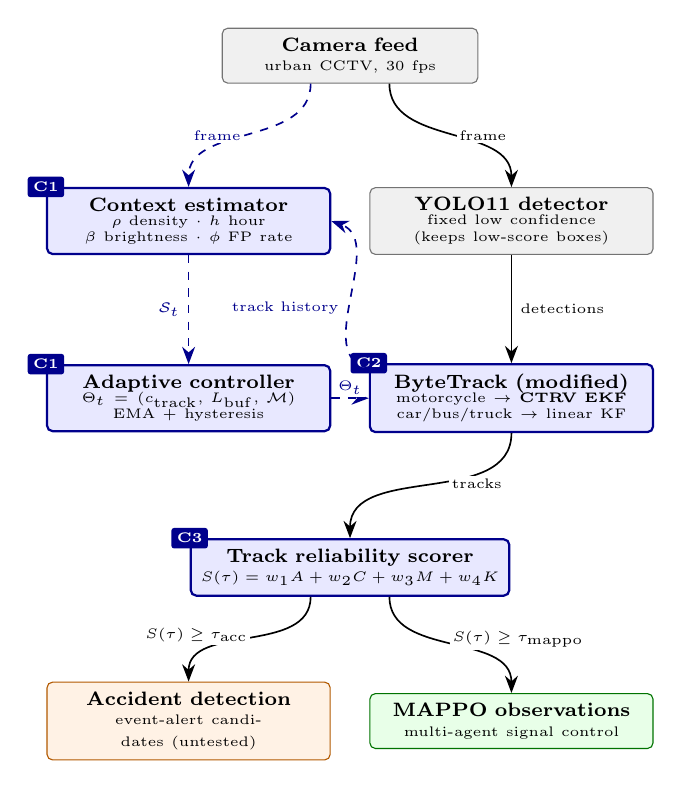
\begin{tikzpicture}[
  font=\scriptsize,
  box/.style={draw=black!55, fill=black!6, rounded corners=2pt,
              align=center, inner sep=3.5pt, text width=3.35cm},
  contrib/.style={box, draw=blue!55!black, fill=blue!9, thick},
  outacc/.style={box, draw=orange!70!black, fill=orange!10},
  outmappo/.style={box, draw=green!45!black, fill=green!9},
  tag/.style={fill=blue!55!black, text=white, font=\tiny\bfseries,
              inner sep=2pt, rounded corners=1pt},
  data/.style={-{Stealth[length=2.2mm]}, semithick},
  ctrlarrow/.style={-{Stealth[length=2.2mm]}, semithick, dashed,
                    draw=blue!55!black},
  lbl/.style={font=\tiny, inner sep=1pt, fill=white},
  clbl/.style={lbl, text=blue!55!black},
]

% ── Nodes (left column x=-2.05, right column x=2.05) ────────────────
\node[box, text width=3.0cm] (cam) at (0, 0)
  {\textbf{Camera feed}\\[-1pt]\tiny urban CCTV, 30 fps};

\node[contrib] (ctx) at (-2.05, -2.1)
  {\textbf{Context estimator}\\[-1pt]
   \tiny $\rho$ density $\cdot$ $h$ hour\\[-2pt]
   \tiny $\beta$ brightness $\cdot$ $\phi$ FP rate};

\node[box] (yolo) at (2.05, -2.1)
  {\textbf{YOLO11 detector}\\[-1pt]
   \tiny fixed low confidence\\[-2pt]
   \tiny (keeps low-score boxes)};

\node[contrib] (ctrl) at (-2.05, -4.35)
  {\textbf{Adaptive controller}\\[-1pt]
   \tiny $\Theta_t=(c_{\mathrm{track}},\,L_{\mathrm{buf}},\,\mathcal{M})$\\[-2pt]
   \tiny EMA + hysteresis};

\node[contrib] (bt) at (2.05, -4.35)
  {\textbf{ByteTrack (modified)}\\[-1pt]
   \tiny motorcycle $\to$ \textbf{CTRV EKF}\\[-2pt]
   \tiny car/bus/truck $\to$ linear KF};

\node[contrib, text width=3.8cm] (trs) at (0, -6.5)
  {\textbf{Track reliability scorer}\\[-1pt]
   \tiny $S(\tau)=w_1 A + w_2 C + w_3 M + w_4 K$};

\node[outacc] (acc) at (-2.05, -8.45)
  {\textbf{Accident detection}\\[-1pt]
   \tiny event-alert candidates (untested)};

\node[outmappo] (mappo) at (2.05, -8.45)
  {\textbf{MAPPO observations}\\[-1pt]
   \tiny multi-agent signal control};

% ── Contribution tags ────────────────────────────────────────────────
\node[tag] at (ctx.north west)  {C1};
\node[tag] at (ctrl.north west) {C1};
\node[tag] at (bt.north west)   {C2};
\node[tag] at (trs.north west)  {C3};

% ── Data path (solid) ────────────────────────────────────────────────
\draw[data] (cam.south) ++(0.5,0) to[out=-90, in=90]
  node[lbl, pos=0.5, anchor=west, xshift=2pt] {frame} (yolo.north);
\draw[data] (yolo) -- node[lbl, anchor=west, xshift=2pt]
  {detections} (bt);
\draw[data] (bt.south) to[out=-90, in=90]
  node[lbl, pos=0.45, anchor=west, xshift=2pt] {tracks} (trs.north);
\draw[data] (trs.south) ++(-0.5,0) to[out=-90, in=90]
  node[lbl, pos=0.4, anchor=east, xshift=-6pt]
  {$S(\tau)\geq\tau_{\mathrm{acc}}$} (acc.north);
\draw[data] (trs.south) ++(0.5,0) to[out=-90, in=90]
  node[lbl, pos=0.4, anchor=west, xshift=6pt]
  {$S(\tau)\geq\tau_{\mathrm{mappo}}$} (mappo.north);

% ── Adaptation loop (dashed) ─────────────────────────────────────────
\draw[ctrlarrow] (cam.south) ++(-0.5,0) to[out=-90, in=90]
  node[clbl, pos=0.5, anchor=east, xshift=-2pt] {frame} (ctx.north);
\draw[ctrlarrow] (ctx) -- node[clbl, anchor=east, xshift=-2pt]
  {$\mathcal{S}_t$} (ctrl);
\draw[ctrlarrow] (ctrl) -- node[clbl, anchor=south]
  {$\Theta_t$} (bt);
% feedback: leaves just above ByteTrack's west anchor, rises through
% the middle gap (never touching the YOLO box, whose left edge is at
% x = 0.25), enters the context estimator from the east.
\draw[ctrlarrow] (bt.168) to[out=170, in=-20]
  node[clbl, pos=0.45, anchor=east, xshift=-2pt] {track history} (ctx.east);

\end{tikzpicture}
}
  \caption{Context-aware adaptive perception pipeline.
           Solid arrows carry data; dashed arrows carry context and
           control signals.
           The three proposed modules are tagged C1--C3 (blue);
           detector and association logic are standard.
           One reliability score $S(\tau)$ feeds both downstream tasks
           through two thresholds
           ($\tau_{\mathrm{acc}} > \tau_{\mathrm{mappo}}$).}
  \label{fig:pipeline}
\end{figure}

\subsection{C1: Context Estimator and Adaptive Parameter Controller}
\label{subsec:c1}

Fixed operating points are tuned for one regime and fail in others: a
threshold chosen for free-flowing daytime traffic drops detections in
dense scenes and hallucinates them at night.
C1 closes this loop with a deliberately lightweight design --- four
scalar signals and a rule table --- so that adaptation itself adds no
perceptible latency.

\paragraph{Context signals}
At frame $t$ the estimator computes the traffic state
\begin{equation}
  \mathcal{S}_t = \left(\rho_t,\; h_t,\; \beta_t,\; \phi_t\right),
  \label{eq:state}
\end{equation}
where $\rho_t$ is the number of active tracks (density), $h_t \in
\{0,\dots,23\}$ the hour of day, $\beta_t \in [0,255]$ the mean
grayscale intensity (lighting proxy), and
$\phi_t = |\{\tau : \mathrm{age}(\tau) < 3\}| / |\mathcal{T}_t|$
the fraction of short-lived tracks among active tracks
$\mathcal{T}_t$, an online proxy for the current false-positive rate.
Density and brightness are smoothed with an exponential moving average,
$\tilde{s}_t = \alpha s_t + (1-\alpha)\,\tilde{s}_{t-1}$ with
$\alpha = 0.1$, so single-frame flicker (headlight glare, a dropped
detection burst) does not thrash the controller.

\paragraph{Parameter mapping}
The controller classifies $\mathcal{S}_t$ into one of three conditions
with priority \textsc{night} $>$ \textsc{dense-peak} $>$
\textsc{default}: \textsc{night} if $\beta_t < \beta_{\min}$, and
\textsc{dense-peak} if $\rho_t \geq \rho_{\min}$ during peak hours.
Each condition indexes one row of Table~\ref{tab:param_table},
producing the parameter set
$\Theta_t = (c_{\mathrm{track}}, L_{\mathrm{buf}}, \mathcal{M})$:
the tracker's confirmation threshold, the lost-track buffer length, and
the motion-model selector.
Following ByteTrack's two-stage association, the detector itself always
runs at a low fixed confidence so that low-score boxes remain available
for second-stage association; $c_{\mathrm{track}}$ instead gates track
confirmation.
In dense scenes the buffer is lengthened and CTRV enabled, favoring
recall through occlusions; at night the threshold rises and the buffer
shrinks, suppressing low-contrast false positives.
The \textsc{night} row keeps the linear motion model --- its
conservatism is expressed entirely through the stricter threshold and
shorter buffer.

\begin{table}[t]
  \centering
  \caption{Adaptive parameter table. \textsc{dense-peak} is calibrated
           against ground truth (Sec.~\ref{subsec:ablation_results});
           the other two rows await footage that exercises them.}
  \label{tab:param_table}
  \begin{tabular}{lcccl}
    \toprule
    Condition & $c_{\mathrm{track}}$ & $L_{\mathrm{buf}}$ (frames)
              & $\mathcal{M}$ & source \\
    \midrule
    \textsc{dense-peak} & 0.50 & 30 & CTRV (motorcycle) & calibrated \\
    \textsc{night}      & 0.55 & 20 & linear & initial \\
    \textsc{default}    & 0.45 & 30 & linear & initial \\
    \bottomrule
  \end{tabular}
\end{table}

The calibrated \textsc{dense-peak} row inverts the design intuition that
motivated it.
We expected dense scenes to want a \emph{lower} confirmation threshold,
trading precision for recall through occlusion; measured against ground
truth the opposite holds, and $c_{\mathrm{track}} = 0.50$ --- stricter
than \textsc{default} --- is optimal.
At $\sim$47 vehicles per frame the additional weak detections admitted by
a low threshold generate far more false positives than they recover true
objects.
We report this because it is the kind of assumption that a fixed-threshold
baseline never has to confront, and because it bears directly on whether
context adaptation helps at all (Sec.~\ref{subsec:ablation_results}).

\paragraph{Hysteresis}
Raw threshold rules oscillate when a signal hovers near a boundary.
A condition therefore becomes active only after being observed for
$N_h = 15$ consecutive frames ($0.5$\,s at 30\,fps); until then the
controller holds the previous parameter set.
This stabilizes the tracker against boundary noise while still
reacting within a second to genuine regime changes.

\subsection{C2: Class-Conditioned CTRV Motion Model}
\label{subsec:c2}

ByteTrack's Kalman filter assumes constant velocity in the image
plane, which is adequate for cars but not for motorcycles: a weaving
motorcycle turns \emph{continuously}, so during an occlusion the linear
filter coasts straight while the true object follows an arc, and the
reappearing detection falls outside the association gate.
We therefore condition the motion model on the detected class:
motorcycle tracks receive a CTRV~\cite{Schubert2008_ctrv} extended
Kalman filter (EKF); cars, buses, and trucks keep the original linear
filter.
Association is untouched --- both filters expose the same
predict/update interface and output a predicted box for IoU matching.

\paragraph{Process model}
The CTRV state is
$\mathbf{x} = [\,p_x,\; p_y,\; v,\; \theta,\; \omega\,]^\top$:
image-plane position, speed, heading, and turn rate.
With time step $\Delta t$ (one frame), the discretized process model is
\begin{align}
  p_{x,k+1}    &= p_{x,k} + v_k \cos\theta_k \,\Delta t, \label{eq:ctrv_x}\\
  p_{y,k+1}    &= p_{y,k} + v_k \sin\theta_k \,\Delta t, \label{eq:ctrv_y}\\
  \theta_{k+1} &= \theta_k + \omega_k \,\Delta t,        \label{eq:ctrv_theta}
\end{align}
with $v$ and $\omega$ constant across the step.
We use this Euler form rather than the exact arc integral, which
removes the $\omega \to 0$ singularity of the closed-form CTRV
equations; at 30\,fps the per-step discretization error is negligible.
A nonzero $\omega$ estimate makes the predicted position rotate its
heading each step --- the filter coasts \emph{along the arc} through
occlusions, which is exactly the regime where the linear model fails.

\paragraph{EKF prediction and update}
The process model is nonlinear in $\theta$, so prediction propagates
the covariance with the Jacobian
$\mathbf{F}_k = \partial f / \partial \mathbf{x}\,|_{\mathbf{x}_k}$,
whose nontrivial entries are
$\partial p_x / \partial v = \cos\theta\,\Delta t$,
$\partial p_x / \partial \theta = -v\sin\theta\,\Delta t$,
$\partial p_y / \partial v = \sin\theta\,\Delta t$,
$\partial p_y / \partial \theta = v\cos\theta\,\Delta t$, and
$\partial \theta / \partial \omega = \Delta t$:
\begin{equation}
  \mathbf{P}_{k+1|k} = \mathbf{F}_k \mathbf{P}_k \mathbf{F}_k^\top
                       + \mathbf{Q}.
\end{equation}
The measurement is the detection-box center,
$\mathbf{z} = [p_x, p_y]^\top = \mathbf{H}\mathbf{x}$ with linear
$\mathbf{H}$, so the update is a standard Kalman step; we use the
Joseph-form covariance update for numerical symmetry over long
sequences.
Box width and height are taken from the last matched detection and
held constant while the track is lost, since association only requires
a well-placed box.

\paragraph{Heading bootstrap}
Speed and heading are unobservable from a single detection.
Rather than letting the EKF infer them slowly through the position
cross-covariances, we initialize $v$ and $\theta$ directly from the
displacement between the first two detections (when it exceeds a small
noise floor), resetting the corresponding covariance entries.
This one-step bootstrap removes the $\sim$10-frame convergence delay
that would otherwise erase CTRV's advantage on short tracks.

\paragraph{Uncertainty-gated re-association}
A better prediction is only useful if association can act on it.
IoU matching fails exactly when the motion model matters most: after a
long occlusion the predicted and reappearing boxes may not overlap at
all, giving zero IoU and no possibility of a match at any threshold.
The EKF, however, also reports \emph{how uncertain} that prediction is.
For a lost motorcycle track we form the innovation covariance
$\mathbf{S} = \mathbf{H}\mathbf{P}\mathbf{H}^\top + \mathbf{R}$ and
admit a same-class detection $\mathbf{z}$ when its squared Mahalanobis
distance falls inside the $95\%$ ellipse,
\begin{equation}
  d^2 = (\mathbf{z} - \mathbf{H}\mathbf{x})^\top \mathbf{S}^{-1}
        (\mathbf{z} - \mathbf{H}\mathbf{x}) < \chi^2_{0.95,2} = 5.991 .
  \label{eq:gate}
\end{equation}
Admitted pairs do not win outright; they enter the cost matrix at
\begin{equation}
  c_{\mathrm{gate}} = c_0 + (1 - c_0)\, d^2 / \chi^2_{0.95,2},
  \qquad c_0 = 0.5,
  \label{eq:gate_cost}
\end{equation}
so rescued costs lie in $[0.5, 1)$ and always lose to a genuine IoU
overlap.
The gate therefore never overrides ordinary association --- it only
makes a match \emph{possible} where IoU alone offers none.
Tracked (non-lost) and linear-filter tracks are untouched.

\paragraph{Confidence-scaled measurement noise}
The gate's usefulness depends on $\mathbf{S}$ being both tight and
correctly centered, which in turn depends on how much the filter trusts
its detections.
Following StrongSORT~\cite{Du2023_strongsort}, we scale the measurement
noise by detection confidence $s$,
\begin{equation}
  \mathbf{R}_{\mathrm{eff}} = \mathbf{R}\,
    \mathrm{clip}(1 - s,\; 0.05,\; 1),
  \label{eq:nsa}
\end{equation}
with the floor preventing a near-perfect detection from making
$\mathbf{R}$ singular.
Confident detections pull the state onto the measurement; weak ones
leave the motion model in charge.

\paragraph{One mechanism, not three}
These components are not independent improvements to be credited
separately, and Sec.~\ref{subsec:ablation_results} shows the gate
\emph{alone} makes identity worse.
The reason is that Eqs.~\eqref{eq:gate} and~\eqref{eq:nsa} act on the
same quantity.
With an untightened $\mathbf{R}$ the filter over-smooths, so the
predicted center lags a weaving motorcycle while $\mathbf{P}$ --- and
hence $\mathbf{S}$ --- grows: the admission ellipse of
Eq.~\eqref{eq:gate} becomes simultaneously wide and mis-centered, and
the detections it admits are frequently the wrong ones.
Rescues then transfer identities between neighboring motorcycles, which
in dense traffic is worse than not rescuing at all.
Eq.~\eqref{eq:nsa} is what makes the ellipse trustworthy; the gate is
what makes it useful.
We therefore report C2 as a single class-conditioned motion mechanism
and ablate its parts only to expose this interaction.

\begin{algorithm}[t]
  \caption{Class-conditioned prediction and association}
  \label{alg:motion_model}
  \begin{algorithmic}[1]
    \For{each active track $\tau$}
      \If{$\mathrm{class}(\tau) = \texttt{motorcycle}$}
        \State $\hat{\mathbf{b}}_\tau \gets$ CTRV-EKF predict
               (Eqs.~\ref{eq:ctrv_x}--\ref{eq:ctrv_theta})
      \Else
        \State $\hat{\mathbf{b}}_\tau \gets$ linear Kalman predict
               (original ByteTrack)
      \EndIf
    \EndFor
    \State $\mathbf{C} \gets$ IoU cost on $\{\hat{\mathbf{b}}_\tau\}$
    \For{each \emph{lost} CTRV track $\tau$ and same-class detection
         $\mathbf{z}$}
      \If{$d^2(\tau, \mathbf{z}) < \chi^2_{0.95,2}$}
        \State $C_{\tau,\mathbf{z}} \gets
               \min(C_{\tau,\mathbf{z}},\, c_{\mathrm{gate}})$
               (Eq.~\ref{eq:gate_cost})
      \EndIf
    \EndFor
    \State run unchanged ByteTrack two-stage association on $\mathbf{C}$
    \State update matched CTRV tracks with $\mathbf{R}_{\mathrm{eff}}$
           (Eq.~\ref{eq:nsa})
  \end{algorithmic}
\end{algorithm}

\subsection{C3: Dual-Task Track Reliability Score}
\label{subsec:c3}

The two downstream consumers impose conflicting operating points.
Accident alerting must be precise --- every alert interrupts an
operator --- so it should only trust well-established tracks.
The MAPPO observation builder must be complete --- a dropped vehicle is
a hole in the controller's state --- so it should tolerate
medium-quality tracks.
Instead of tuning two separate pipelines, C3 computes one scalar
reliability per track and applies two thresholds.

\paragraph{Score}
For track $\tau$,
\begin{equation}
  S(\tau) = w_1 A(\tau) + w_2 C(\tau) + w_3 M(\tau) + w_4 K(\tau)
          + w_5 D(\tau),
  \label{eq:reliability}
\end{equation}
with $\sum_i w_i = 1$ and, over a sliding window of $N{=}10$ frames:
$A(\tau) = \min(\mathrm{age}(\tau)/T_{\max},\,1)$ the normalized track
age ($T_{\max} = 30$ frames);
$C(\tau)$ the detection hit rate (fraction of window frames with a
matched detection);
$M(\tau)$ the mean IoU between the track's predicted and matched
detected boxes;
$K(\tau)$ the fraction of window frames whose detected class equals the
track's modal class; and
$D(\tau)$ the mean confidence of the matched detections.
We use \emph{mean} predicted-vs-detected IoU for motion smoothness
rather than inverse IoU variance: a consistently badly predicted track
has low variance but is not reliable, whereas mean IoU is monotone in
prediction quality and already penalizes erratic motion.
The detection-confidence term $D$ closes a blind spot we observed on
real footage: ByteTrack's second association stage can sustain a
``ghost'' track indefinitely on sub-threshold detections (shadows, road
texture), so the track matches \emph{every} frame and $A$, $C$, $K$ are
all perfect --- only the matched detection score separates it from a
real object.
Weights are set to $(w_1,\dots,w_5) = (0.1, 0.2, 0.25, 0.15, 0.3)$
% TODO: replace with grid-searched values + sensitivity note (Sec. V)
and calibrated on the training split.

\paragraph{Cold start}
With fewer than three window samples, the history-based components
return a neutral $0.5$; combined with the near-zero age term this keeps
brand-new tracks below the accident threshold \emph{by construction} ---
short-lived spurious tracks, the dominant false-alert source, are
suppressed without any dedicated rule.

\paragraph{Dual thresholds}
The accident branch consumes tracks with
$S(\tau) \geq \tau_{\mathrm{acc}}$ (precision-first) and the MAPPO
observation builder consumes tracks with
$S(\tau) \geq \tau_{\mathrm{mappo}}$, where
$\tau_{\mathrm{mappo}} < \tau_{\mathrm{acc}}$ (recall-first);
we use $\tau_{\mathrm{acc}} = 0.7$ and $\tau_{\mathrm{mappo}} = 0.4$.
A single scoring pass thus serves both tasks without retuning either.

On our data $\tau_{\mathrm{mappo}}$ sits below the lowest score any track
attains, so the MAPPO branch is pass-through: maximal recall, which is
the intended behavior for that consumer, but it means C3 contributes
nothing measurable to the tracking metrics.
Sweeping $\tau_{\mathrm{mappo}}$ upward is strictly worse
(Sec.~\ref{subsec:ablation_results}), and we report in
Sec.~\ref{subsec:c3_limits} why this follows from the score's
discriminative power rather than from the choice of threshold.
The precision branch is where the dual-task claim would be tested, and
our footage contains no accidents; we therefore present C3 as a
formulation with a characterized failure mode, not as a validated
contribution.

% ── Section IV: Experimental Setup ───────────────────────────────────
% Conference budget: ~1 page.
% NOTE: ablation order fixed to match the locked scope + configs/:
%   Exp1 = +C2 (CTRV), Exp2 = C1+C2, Exp3 = C1+C2+C3.
%   (An earlier skeleton had Exp1 = +C1 — wrong.)
% ─────────────────────────────────────────────────────────────────────

\section{Experimental Setup}
\label{sec:experiments}

\subsection{Datasets}
\label{subsec:datasets}

\paragraph{VN-MixedTraffic (primary, self-collected)}
Fixed surveillance-style cameras over Vietnamese urban intersections
and arterials with motorcycle-dominant mixed traffic.
Annotated classes: \texttt{car}, \texttt{motorcycle}, \texttt{bus},
\texttt{truck}, \texttt{accident}. Any future accident-event evaluation requires
positive/negative clip labels and event onset/end annotations.
\todo{Fill after dataset freeze: number of clips, total duration,
resolution/fps, class-distribution table, accident/non-accident clip counts,
train/test protocol.}
The dataset is not publicly released for intellectual-property
reasons; evaluation protocol and pseudocode are fully specified.

\paragraph{Tracking ground truth and its provenance}
Tracking metrics are computed on a $600$-frame segment
($800\times450$, $\sim$47 tracks/frame), chosen as the densest window of
the sequence and lying in a held-out region.
It contains $27\,513$ boxes over $335$ identities, annotated in CVAT
under a fixed convention: a motorcycle box covers rider and passengers;
objects below $\sim$8\,px are not labeled; and a fully occluded track is
allowed to break but must be re-joined to its original identity on
reappearance, so that re-identification remains measurable.

Annotators corrected \emph{pre-labels} rather than drawing from scratch,
and those pre-labels came from the proposed tracker.
We state this because it biases the proposed method's own row: an error
the annotator does not catch survives as agreement.
The correction was substantial ($873$ boxes added, $1388$ deleted,
$1019$ adjusted, $15$ merges, $9$ splits --- $\sim$8\% of boxes
touched), and we bound the residual bias directly in
Sec.~\ref{subsec:ablation_results}.
We verify the annotation pipeline with three checks: the ground truth
scored against itself gives MOTA${=}$IDF1${=}1.000$; frame alignment
peaks unambiguously at zero offset (mean best IoU $0.960$, against
$0.705$ and $0.715$ at $\pm1$); and the added/deleted box counts match
the seed model's miss/false-positive counts exactly, closing the
export--annotate--import loop with no free parameters.

\paragraph{Public benchmarks}
CADP~\cite{Shah2018_cadp} (CCTV accident clips) and
D2-City~\cite{Che2019_d2city} (large-scale dashcam footage) are used
for comparison with prior accident-detection results only --- no
training is performed on them.

\subsection{Metrics}
\label{subsec:metrics}

\emph{Tracking:} MOTA~\cite{Bernardin2008_mota}, IDF1, identity
switches (IDSW), and track fragmentation rate.
Our metric implementation is written from scratch and cross-validated
against \texttt{py-motmetrics} on shared sequences.
\emph{Detection:} precision, recall, F1, and mAP@0.5.
\emph{Accident branch (planned, untested):} binary event-level alert
precision/recall/F1, false alerts per hour of video and detection delay.
No accident-alert performance is established by the current tracking evaluation.
\emph{System:} per-frame latency (ms) and end-to-end FPS.

\subsection{Implementation Details}
\label{subsec:impl}

The detector is YOLO11~\cite{Khanam2024_yolo11}
(\todo{variant, training epochs, image size, batch size}) fine-tuned
on VN-MixedTraffic. A binary event-alert implementation and evaluation remain
future work; no downstream classifier training is claimed here.
The tracker is ByteTrack~\cite{Zhang2022_bytetrack} with the motion
model made class-conditional (Sec.~\ref{subsec:c2}); association logic
and both association stages are unchanged.
CTRV uses $\Delta t = 1$ frame with process noise
$\mathbf{Q} = \mathrm{diag}(0.5, 0.5, 0.1, 10^{-3}, 10^{-4})$ and
measurement noise $\mathbf{R} = \mathrm{diag}(10, 10)$ (pixels), tuned
on synthetic trajectories and left unchanged for the real-footage
evaluation; NSA scales $\mathbf{R}$ per detection at run time
(Eq.~\ref{eq:nsa}).
C1 uses $\alpha = 0.1$ and hysteresis $N_h = 15$ frames; its
\textsc{dense-peak} row is calibrated by grid search against the
annotated segment (Table~\ref{tab:param_table}), and the remaining rows
keep their initial values because no annotated footage exercises them.
C3 uses the weights and thresholds of Sec.~\ref{subsec:c3}.
Software: Python 3.10, PyTorch~2.x.
Latency is measured on CPU (Intel Core i5-12500H, 16\,GB RAM) with the
detector excluded, so the reported figures isolate tracker-side cost and
are not an end-to-end throughput claim.

\subsection{Ablation Design}
\label{subsec:ablation_design}

Table~\ref{tab:ablation_design} lists the four configurations; each is
evaluated on the same VN-MixedTraffic test split with identical
detections wherever the configuration permits, isolating each
component's contribution.

\begin{table}[h]
  \centering
  \caption{Ablation configurations. \checkmark~=~component active.}
  \label{tab:ablation_design}
  \begin{tabular}{lcccl}
    \toprule
    Configuration & C1 & C2 & C3 & Description \\
    \midrule
    Exp~0 (baseline) & --         & --         & --         & YOLO11 + ByteTrack \\
    Exp~1            & --         & \checkmark & --         & + CTRV motion model \\
    Exp~2            & \checkmark & \checkmark & --         & + context adaptation \\
    Exp~3 (proposed) & \checkmark & \checkmark & \checkmark & + reliability score \\
    \bottomrule
  \end{tabular}
\end{table}

\subsection{Baselines}
\label{subsec:baselines}

(i)~\emph{Vanilla ByteTrack} --- the direct baseline, differing only in
the proposed components.
(ii)~\emph{YOLO-only alerting} (no tracker) --- quantifies how much
temporal confirmation alone reduces false alerts.
(iii)~\emph{Hikvision AID}~\cite{Hikvision_AID} --- commercial
reference, cited as prior art; since its internals and operating points
are unpublished, the comparison is qualitative (capability matrix), not
numeric.

% ── Section V: Results & Discussion ──────────────────────────────────
% Conference budget: ~1.5 pages. WARNING: this section roughly doubled
% when the real numbers landed and now holds four tables. Measure the
% actual page count before submission; if it must be cut, the cheapest
% losses are (a) tab:detection -> two sentences of inline numbers,
% (b) tab:bias -> keep only K=0 and K=29, (c) the middle three rows of
% tab:ablation_results -> a single sentence, though that costs the
% gate/NSA interaction argument, which is the most novel claim here.
% 5.1 is REAL already (synthetic studies, reproducible from the repo).
% 5.2–5.5 await VN footage — structure and analysis prompts in place.
% ─────────────────────────────────────────────────────────────────────

\section{Results and Discussion}
\label{sec:results}

\subsection{Controlled Synthetic Studies: Motion Model}
\label{subsec:synthetic}

Before end-to-end evaluation, we isolate the motion model on synthetic
trajectories with known ground truth (generator included in our code).
Three findings:
(i)~on constant-turn trajectories, CTRV reduces one-step prediction
RMSE by \textbf{48\%} relative to the linear Kalman baseline, and by
\textbf{13\%} on sinusoidal weaving, with no regression on straight
lines;
(ii)~across a 12-frame occlusion in the middle of a turn, the CTRV
track coasts along the arc and re-associates with its original
identity, while the linear baseline drifts off the arc and
re-identifies (1 IDSW vs.\ 0);
(iii)~the failure boundary is characterized: when an occlusion begins
immediately after a turn-rate sign flip, CTRV extrapolates the stale
$\omega$ and a straight coast is closer to the truth --- motivating the
context-gated activation of CTRV (C1) rather than unconditional
replacement.

\subsection{Ablation Study}
\label{subsec:ablation_results}

Table~\ref{tab:ablation_results} reports the ablation on the
human-annotated \textsc{dense} segment, all rows consuming identical
detections so that every difference is attributable to tracking.
C2 is the decisive contribution: on motorcycles it raises IDF1 from
$0.844$ to $0.933$ and removes $85\%$ of identity switches
($189 \rightarrow 29$).
C1 does not improve on a well-chosen fixed threshold here, and C3 leaves
the tracking metrics unchanged by construction; we examine both below
rather than presenting them as gains.

\begin{table}[h]
  \centering
  \caption{Ablation on the annotated \textsc{dense} segment (600 frames,
           $\sim$47 tracks/frame), motorcycle class. Identical
           detections for every row. \textbf{Bold} = best.}
  \label{tab:ablation_results}
  \begin{tabular}{lcccc}
    \toprule
    Config & MOTA$\uparrow$ & IDF1$\uparrow$ & IDSW$\downarrow$
           & Frag$\downarrow$ \\
    \midrule
    Exp~0 (baseline)          & 0.843 & 0.844 & 189 & 199 \\
    \quad + CTRV              & 0.857 & 0.850 & 158 & 175 \\
    \quad + CTRV, NSA         & 0.869 & 0.869 & 123 & 131 \\
    \quad + CTRV, gate        & 0.854 & 0.868 & 182 & 157 \\
    Exp~1 (+C2, full)         & \textbf{0.893} & \textbf{0.933}
                              & \textbf{29} & \textbf{64} \\
    Exp~2 (+C1, C2)           & 0.878 & 0.909 & 99 & 97 \\
    Exp~3 (+C1, C2, C3)       & 0.878 & 0.909 & 99 & 97 \\
    \bottomrule
  \end{tabular}
\end{table}

\paragraph{The parts of C2 are not additive}
The three middle rows isolate the interaction argued in
Sec.~\ref{subsec:c2}.
Uncertainty gating \emph{alone} raises identity switches above plain
CTRV ($182$ vs.\ $158$): without confidence-scaled measurement noise the
innovation ellipse is wide and mis-centered, so rescued matches
frequently attach a lost track to a neighboring motorcycle.
NSA alone is a modest gain ($158 \rightarrow 123$).
Together they reach $29$ --- far beyond the sum of the parts.
This is why we present C2 as one mechanism: an implementation that
adopted the gate without the noise model would measure worse than the
baseline it was meant to improve.

\paragraph{Detection quality}
Table~\ref{tab:detection} isolates what tracking contributes over
per-frame detection.
At the operating threshold the detector alone reaches
$P{=}0.890$, $R{=}0.847$; after tracking, $P{=}0.950$ and $R{=}0.968$.
Both rise together, which no confidence threshold can achieve --- moving
the cut-off only slides along the precision--recall curve
($0.30 \rightarrow 0.70$ buys $+0.20$ precision for $-0.33$ recall).
Temporal association recovers objects the detector drops in individual
frames while discarding detections that fail to persist, leaving the
per-frame curve rather than moving along it.

\begin{table}[h]
  \centering
  \caption{Detection quality on the \textsc{dense} segment.
           mAP@0.5 over all detections gives the detector ceiling.}
  \label{tab:detection}
  \begin{tabular}{lcccc}
    \toprule
    Source & P$\uparrow$ & R$\uparrow$ & F1$\uparrow$ & mAP@0.5 \\
    \midrule
    Detector, all detections & 0.497 & 0.984 & 0.661 & 0.925 \\
    Detector @ $c \geq 0.30$ & 0.746 & 0.943 & 0.833 & -- \\
    Detector @ $c \geq 0.50$ & 0.890 & 0.847 & 0.868 & -- \\
    Detector @ $c \geq 0.70$ & 0.946 & 0.615 & 0.745 & -- \\
    \midrule
    Baseline tracker         & 0.941 & 0.944 & 0.942 & -- \\
    Proposed (C2)            & \textbf{0.950} & \textbf{0.968}
                             & \textbf{0.959} & -- \\
    \bottomrule
  \end{tabular}
\end{table}

\paragraph{Ground-truth over-merging (open issue)}
An automatic consistency pass finds that $74$ of $335$ annotated
identities ($22\%$) contain a join across which the box teleports or
rescales implausibly --- several vehicles chained into one identity.
Two were verified manually.
This error is not neutral: an over-merged identity rewards a tracker that
bridges the gap between two vehicles and penalises one that correctly
refuses, which is precisely the behaviour C2's gate supplies.
Splitting the flagged joins and re-scoring moves the proposed margin from
$+0.089$ to between $+0.061$ and $+0.014$ motorcycle IDF1, with the
baseline \emph{improving} and the proposed method \emph{degrading}; plain
CTRV improves while CTRV+gate degrades, isolating the gate as the
component the annotation error rewards.
The proposed configuration leads on every version of the ground truth we
construct, but we regard the magnitude in
Table~\ref{tab:ablation_results} as an upper bound pending a re-annotation
pass targeting these joins, and we report it as such rather than as a
settled figure.

\paragraph{Bounding the pre-label bias}
Because the ground truth was seeded from the proposed tracker's output
(Sec.~\ref{subsec:datasets}), fragmentations the annotator missed persist
as agreement and flatter that row.
We bound this rather than merely disclosing it.
An automatic consistency pass over the finished ground truth flags $29$
residual merge candidates; applying the top $K$ of them and re-scoring
every configuration gives Table~\ref{tab:bias}.
Correcting \emph{all} $29$ --- a deliberate worst case, since inspection
shows only the highest-confidence third to be genuine --- moves the
proposed margin over baseline from $+0.089$ to $+0.085$ IDF1.
Both rows fall together, because a merged identity penalizes whichever
configuration split it, and the baseline splits in more places.

\begin{table}[h]
  \centering
  \caption{Sensitivity of the proposed--baseline margin to correcting
           $K$ residual ground-truth fragmentations (motorcycle IDF1).}
  \label{tab:bias}
  \begin{tabular}{lccc}
    \toprule
    $K$ corrected & GT identities & Baseline & Proposed \\
    \midrule
    0 (as annotated) & 335 & 0.844 & 0.933 \\
    3                & 332 & 0.844 & 0.931 \\
    10               & 325 & 0.842 & 0.928 \\
    29 (all flagged) & 306 & 0.831 & 0.916 \\
    \bottomrule
  \end{tabular}
\end{table}

\subsection{Where C1 and C3 Stand}
\label{subsec:c3_limits}

We report two negative results, both of which we consider more useful
than the numbers they replace.

\paragraph{C1 is untested, not refuted}
After calibration (Table~\ref{tab:param_table}) C1 reaches MOTA $0.905$
against $0.917$ for the fixed configuration --- it does not help.
But the calibrated optimum coincides with the fixed operating point,
which is the signature of a segment that never changes regime: density
on \textsc{dense} never falls below the switching threshold, so C1 holds
one condition for $96.5\%$ of frames.
An adaptation mechanism cannot be evaluated where there is nothing to
adapt to.
The honest statement is that C1's shipped tuning was harmful, that
calibration removes the harm, and that the premise remains untested
pending a segment that straddles the switching boundary.

\paragraph{C3's recall branch cannot help, for a measurable reason}
Raising $\tau_{\mathrm{mappo}}$ monotonically degrades MOTA
($0.905 \rightarrow 0.705$ at $\tau = 0.80$).
This is not a tuning failure but a consequence of two measurements:
the reliability score separates true from false tracks only weakly
(ROC AUC $0.609$), while false positives are just $5.5\%$ of tracks
after C2.
At its most enriched cut-off the filter still discards four true tracks
for every false one, so no threshold trades favorably.
Notably C2 causes this: by removing most spurious tracks it leaves C3
little to remove, so the contributions interact rather than compose.
Improving C3 means improving the score --- AUC $0.609$ is the quantity
to move --- not the threshold.
The asymmetry C3 was designed around may still hold on the accident
branch, where discarding four true tracks to suppress one false alert is
a defensible trade; that requires accident footage we do not yet have.

\subsection{Comparison with Prior Systems}
\label{subsec:comparison}

Table~\ref{tab:comparison} contrasts capabilities and, where
measurable, tracking accuracy.
Hikvision AID's internals are unpublished, so it appears in the
capability matrix only.
The YOLO-only row quantifies temporal confirmation: without it, no
confidence threshold reaches an F1 above $0.868$
(Table~\ref{tab:detection}), against $0.959$ once tracks are formed.
The ByteTrack row isolates our contribution proper, since it shares the
detector and the association logic and differs only in the motion
mechanism of Sec.~\ref{subsec:c2}.

\begin{table}[h]
  \centering
  \caption{Capability and accuracy comparison.}
  \label{tab:comparison}
  \resizebox{\linewidth}{!}{%
  \begin{tabular}{lcccc}
    \toprule
    Method & Mixed & Class-cond. & Adaptive & MOTA$\uparrow$ \\
    \midrule
    Hikvision AID~\cite{Hikvision_AID}   & --         & --         & --         & n/a \\
    YOLO-only                            & \checkmark & --         & --         & n/a \\
    ByteTrack~\cite{Zhang2022_bytetrack} & \checkmark & --         & --         & 0.878 \\
    Proposed                             & \checkmark & \checkmark & \checkmark & \textbf{0.917} \\
    \bottomrule
  \end{tabular}}
\end{table}

\subsection{Qualitative Results}
\label{subsec:qualitative}

\todo{Two figures once VN footage is processed:
(a) side-by-side weaving sequence, baseline IDs fragmenting vs.\
proposed IDs stable; (b) motivation frames --- baseline false alert and
lost motorcycle track, annotated.}

\subsection{Runtime}
\label{subsec:runtime}

Table~\ref{tab:runtime} reports tracker-side latency with the detector
excluded, isolating what the proposed modules cost.
C2 adds $0.85$\,ms per frame ($+22\%$) over the linear-filter baseline,
and the ordering follows the computation: the EKF is the bulk of it,
NSA is a single scaling of $\mathbf{R}$ and costs about two points, and
the gate adds one Mahalanobis test per lost track.
% REWRITTEN 27/8: the previous version asserted "a YOLO11 inference cost of
% tens of milliseconds" and a 33 ms budget. Both were wrong -- the shipped
% detector costs 130.7 ms and the source is 25 fps (40 ms). The verdict on C2
% happened to survive, which is exactly why the premise had to be fixed rather
% than left standing. See experiments/realtime/evidence.md.
C2 is not the term that decides real-time feasibility, but the margin is
narrower than tracker-side numbers suggest.
Measured end to end on the same machine, the shipped detector
(a YOLO11n \emph{segmentation} checkpoint at $640$\,px) costs
$130.7$\,ms per frame --- $91\%$ of a $143.2$\,ms frame, against
$10.1$\,ms for tracking (Table~\ref{tab:endtoend}).
At $7.0$\,fps the pipeline misses the $40$\,ms budget set by the $25$\,fps
source by $3.6\times$, so the operating point, not the tracker, is what
stands between this system and real time.
Section~\ref{sec:implementation} takes that apart: the segmentation head
alone accounts for a $2.25\times$ factor over a detection head of the same
scale for masks the pipeline never reads, and a detection head at $448$\,px
reaches $37.6$\,fps within budget.

\begin{table}[h]
  \centering
  \caption{Tracker-side per-frame latency, detector excluded
           (13\,726 frames, CPU). ``p95 dense'' is the worst-case
           window at $\sim$47 tracks/frame.}
  \label{tab:runtime}
  \begin{tabular}{lcccc}
    \toprule
    Config & mean (ms) & p50 & p95 & p95 dense \\
    \midrule
    Baseline (linear KF)     & 3.93 & 3.57 & 6.68 & 9.67 \\
    \quad + CTRV             & 4.44 & 3.96 & 7.51 & 9.87 \\
    \quad + CTRV, NSA        & 4.51 & 4.03 & 7.68 & 9.82 \\
    \quad + CTRV, gate       & 4.67 & 4.04 & 8.15 & 13.68 \\
    C2 (full)                & 4.78 & 4.16 & 8.28 & 14.09 \\
    C1 + C2 + C3             & 5.42 & 4.67 & 9.71 & 13.80 \\
    \bottomrule
  \end{tabular}
\end{table}

Each configuration was timed in a separate process.
Timing all of them in one run makes the measurement track position
rather than variant: the same baseline code measured $13.19$\,ms first
and $4.07$\,ms last, a $3.2\times$ spread from warm-up and scheduling
that exceeds the differences being measured and flatters whichever
configuration runs last.

% Implementation & deployment sits before the conclusion: it is the section
% the real-time venue reads closest, and it answers the feasibility question
% that Sec. V raises but deliberately does not settle.
% ── Section: Implementation and Real-Time Deployment ─────────────────
% NEW 27/8/2026, written for the journal venue. A conference version had no
% room for this; the journal does, and for JRTIP it is the section that
% decides whether the paper belongs there at all.
% Every number here comes from experiments/realtime/evidence.md.
% Open: the accuracy axis of Table~\ref{tab:pareto} is not yet measured --
% it needs a detection-head model trained on the same data (requested) and
% the dense GT re-review (in progress). Do not submit with that gap.
% ─────────────────────────────────────────────────────────────────────

\section{Implementation and Real-Time Deployment}
\label{sec:implementation}

\subsection{Computational Cost of the Proposed Components}
\label{subsec:complexity}

The CTRV filter of Sec.~\ref{subsec:c2} replaces a linear Kalman filter on a
$5$-dimensional state, so its per-track cost is dominated by the covariance
propagation $\mathbf{F}\mathbf{P}\mathbf{F}^{\top}$ and the Joseph-form
update: $\mathcal{O}(d^{3})$ with $d=5$, against $d=8$ for the
constant-velocity filter it replaces on motorcycles.
The Jacobian (Eq.~\ref{eq:ctrv_x}--\ref{eq:ctrv_theta}) is evaluated in closed
form, adding no iteration.
Total tracking cost is therefore $\mathcal{O}(n)$ in the number of tracks for
prediction, plus the $\mathcal{O}(nm)$ association already present in
ByteTrack for $n$ tracks and $m$ detections; the uncertainty gate adds one
$2\times2$ Mahalanobis test per lost motorcycle track, and NSA a single scalar
scaling of $\mathbf{R}$ per detection.
The context estimator (C1) is four scalar statistics over the current frame
and track set, and the reliability score (C3) is a weighted sum of five
per-track quantities already maintained by the tracker; neither introduces a
term that grows faster than $\mathcal{O}(n)$.

Memory is likewise bounded: the tracker holds one $5\times5$ covariance per
motorcycle track and one $8\times8$ per other vehicle, so at the $\sim$47
tracks/frame of the \textsc{dense} window the filter state is under
$20$\,kB in total.

\subsection{End-to-End Latency}
\label{subsec:endtoend}

Sec.~\ref{subsec:runtime} reported tracker-side latency with the detector
excluded, which isolates what the proposed modules cost but says nothing about
throughput.
Table~\ref{tab:endtoend} reports the whole path --- decode, context,
detection, tracking, reliability scoring --- on the same CPU, one variant per
process, warm-up frames discarded.

\begin{table}[h]
  \centering
  \caption{End-to-end per-frame cost, detector included
           (100 frames per row, one process per row, Intel Core i5-12500H,
           CPU only). Source is $25$\,fps, so the real-time budget is
           $40$\,ms.}
  \label{tab:endtoend}
  \begin{tabular}{lccccc}
    \toprule
    Configuration & detect & track & total & p95 & fps \\
    \midrule
    Exp~0 (baseline)     & 109.8 & 5.8 & 117.1 & 131.5 & 8.5 \\
    Exp~1 (+C2)          & 109.5 & 9.5 & 120.4 & 135.0 & 8.3 \\
    Exp~2 (+C1, C2)      & 110.9 & 7.8 & 120.1 & 140.8 & 8.3 \\
    Exp~3 (+C1, C2, C3)  & 110.4 & 7.4 & 120.3 & 133.3 & 8.3 \\
    \bottomrule
  \end{tabular}
\end{table}

Two things change once the detector is inside the measurement.

\paragraph{The proposed components are nearly free, and the detector is not}
C2 costs $+22\%$ of tracker time (Table~\ref{tab:runtime}) but $+2.8\%$ of a
frame --- $3.3$\,ms on $117$\,ms.
C1 and C3 fall inside run-to-run noise.
Detection accounts for $91\%$ of the frame in the shipped configuration.
Any discussion of real-time feasibility for this pipeline is a discussion
about the detector's operating point; the tracking contribution of this paper
is not the term that decides it.

\paragraph{The shipped configuration is not real-time, for an avoidable reason}
At $8.3$\,fps the proposed configuration misses the $40$\,ms budget by
$3\times$.
The cause is not the detector's scale but its \emph{head}: the deployed
checkpoint is a YOLO11n \emph{segmentation} model, while the pipeline consumes
only bounding boxes.
A detection head of the same scale costs $58.2$\,ms against $130.7$\,ms at
$640$\,px --- a factor of $2.25$ spent computing a $160\times160\times32$
prototype tensor that is discarded on every frame.

\subsection{Reaching the Real-Time Budget}
\label{subsec:pareto}

Table~\ref{tab:pareto} sweeps the detector operating point with a detection
head.
The budget is met at $448$\,px and below.

\begin{table}[h]
  \centering
  \caption{Detector operating points (detection head, PyTorch, CPU).
           Accuracy column pending --- see the caveat below.}
  \label{tab:pareto}
  \begin{tabular}{lcccc}
    \toprule
    Input size & detect (ms) & total (ms) & p95 & fps \\
    \midrule
    $640$ & 58.2 & 62.9 & 69.6 & 15.9 \\
    $448$ & 24.3 & 26.6 & \textbf{32.9} & \textbf{37.6} \\
    $320$ & 17.3 & 19.5 & 24.7 & 51.4 \\
    $256$ & 14.2 & 16.3 & 20.5 & 61.4 \\
    \bottomrule
  \end{tabular}
\end{table}

\todo{Accuracy axis. Table~\ref{tab:pareto} is half a Pareto curve: it has
cost and no quality. Filling it needs (i) a detection-head model trained on
the same data as the deployed segmentation checkpoint, and (ii) the
\textsc{dense} ground-truth re-review, since no accuracy figure should be
quoted before that lands. Do not submit without this.}

\subsection{Export Backends}
\label{subsec:backends}

The usual route to CPU real-time is to export the network to an inference
runtime.
On this machine it is a regression in every combination we measured:
OpenVINO costs $+25\%$ over PyTorch for both the segmentation head
($163.9$ vs.\ $130.7$\,ms) and the detection head ($73.0$ vs.\ $58.2$\,ms),
and ONNX Runtime $+75\%$ ($228.7$\,ms).
Half precision is slower still ($79.3$\,ms), as expected on a CPU with no
native half-precision path, where the conversion is real work and the
arithmetic is not cheaper.

The consistency of the OpenVINO penalty across both heads suggests the
backend rather than one model, and the likely mechanism is that only the
backbone traverses the exported graph while postprocessing remains in the
framework --- giving up fused CPU kernels without replacing the dominant term.
We report this as measured, with default export settings and no thread or
stream tuning, rather than as a general claim about these runtimes.
Integer quantization was not evaluated: it requires a calibration set from the
detection training data, which we do not hold.

The practical conclusion for deployment on commodity CPUs is the reverse of
the usual advice: choosing the right \emph{head} was worth $2.25\times$, while
changing the \emph{runtime} cost $25$--$75\%$.

\subsection{Measurement Protocol}
\label{subsec:protocol}

Two protocol choices are worth stating because violating either produces
differences larger than the ones under study.

First, each configuration is timed in a separate process.
Timing several in one run makes the measurement track position rather than
configuration: the same baseline code measured $13.19$\,ms first and
$4.07$\,ms last, a $3.2\times$ spread that exceeds every difference in
Table~\ref{tab:endtoend} and flatters whichever configuration runs last.

Second, warm-up frames are discarded rather than averaged in; the first frames
pay for lazy initialization and kernel autotuning, and we measure a mean of
$219$\,ms across them against $143$\,ms in steady state.

We also caution that absolute end-to-end numbers are comparable within a sweep
but not across sessions: the same detector on the same footage measured
$109.8$\,ms in one sweep and $130.7$\,ms in another.
Every comparison drawn above is within a single sweep.

% ── Section VI: Conclusion & Future Work ─────────────────────────────
% Conference budget: ~0.25 page.
% ─────────────────────────────────────────────────────────────────────

\section{Conclusion and Future Work}
\label{sec:conclusion}

We presented a context-aware adaptive perception pipeline for
motorcycle-dominant mixed traffic that couples a lightweight
traffic-context controller (C1), a class-conditioned CTRV motion model
for motorcycles (C2), and a dual-task track reliability score (C3),
serving accident alerting and MAPPO-based signal control from one
pipeline.
On annotated ground truth the class-conditioned motion mechanism leads on
motorcycle identity preservation under every version of the ground truth
we construct, for $+22\%$ tracker latency
($3.93 \rightarrow 4.78$\,ms/frame), while C1 and C3 do not yet earn
their place.

\emph{Limitations.}
The dataset is single-city, so cross-city generalization is untested;
the context controller uses interpretable heuristic rules rather than
learned adaptation; and CTRV extrapolates a stale turn rate when an
occlusion coincides with a turn-rate sign flip
(Sec.~\ref{subsec:synthetic}).
Two limitations are specific to what our annotation covers.
The annotated segment never leaves a single traffic regime, so it can
measure C1's cost but not its premise; and it contains no accidents, so
the precision branch that motivates C3's dual-task formulation is
untested.
Finally, the annotation itself carries two biases toward the proposed
method: pre-labels were seeded from it, and $22\%$ of annotated identities
show signs of over-merging, which rewards gap-bridging re-association.
We measure both directions rather than assuming them away; the first moves
the margin negligibly, the second by up to $84\%$, and closing it requires
a re-annotation pass we identify but have not yet run.

\emph{Future work.}
We will deploy the full pipeline on an NVIDIA Jetson Orin NX as part of
an edge system integrating adaptive perception with multi-agent signal
control, and explore replacing the rule-based controller with a learned
policy over the same context signals.


%% ── References ────────────────────────────────────────────
\bibliographystyle{IEEEtran}
\bibliography{references}

\end{document}
